\lab{Algorithms}{Introduction to Wavelets}{Intro to Wavelets}

\objective{Learn the basics of Wavelet Analysis 
and explore the wavelet-based FBI fingerprint compression standard.}

Recall that in the context of Fourier analysis, one seeks to represent a
function as a sum of sinusoids. One drawback to this approach is that the
Fourier transform only captures global frequency information, and local 
information is lost; we can know which frequencies are the
most prevalent, but not when they occur. 
The Wavelet transform provides an alternative approach that avoids this shortcoming,
and is often a superior analysis technique for many types of signals and images.

\subsection*{The Discrete Wavelet Transform}
In wavelet analysis, we seek to analyze a function by considering its \emph{wavelet decomposition}.
The wavelet decomposition of a function is a way of expressing the function as a linear combination 
of a particular family of basis functions. 
In this way, we can represent a function by the sequence of coefficients (called 
\emph{wavelet coefficients}) defining this linear combination.
The mapping from a function to its sequence of wavelet coefficients is called the \emph{discrete 
wavelet transform}. 

This situation is entirely analogous to the discrete Fourier transform, differing only in the choice
of basis functions. In Wavelet analysis, we determine the family of basis functions by first starting
off with a function $\psi$ called the \emph{wavelet} and a function $\phi$ called the \emph{scaling function}
(these functions are also called the mother and father wavelets, respectively). We then generate 
the following countable families of basis functions (sometimes called baby wavelets) from these two functions:
\begin{equation*}
\psi_{m,k}(x) = \psi(2^mx - k)
\end{equation*}
\begin{equation*}
\phi_{m,k}(x) = \phi(2^mx - k),
\end{equation*}
where $m,k \in \mathbb{Z}$.

The historically first, and most basic, wavelet is called the \emph{Haar Wavelet},
given by
\[
\psi(x) =
 \begin{cases}
  1 & \text{if } 0 \leq x < \frac{1}{2} \\
  -1 & \text{if } \frac{1}{2} \leq x < 1 \\
  0 & \text{otherwise.}
 \end{cases}
\]
% It might be nice to plot this function and include the image in the lab.
The associated scaling function is given by
\[
\phi(x) =
 \begin{cases}
 1 & \text{if } 0 \leq x < 1 \\
 0 & \text{otherwise.}
 \end{cases}
\]

Let's launch into an implementation of the one-dimensional discrete wavelet transform.
Our solution will be an iterative algorithm that successively computes more and more coefficients.
The key operations in the algorithm are the discrete convolution ($*$) and down-sampling ($\downarrow$).
The inputs to the algorithm are a one-dimensional array $X$ (the signal that we want to transform), a one-dimensional
array $L$ (called the \emph{low-pass filter}), a one-dimensional array $H$ (the \emph{high-pass filter}), and a positive
integer $n$ (controlling to what degree we wish to transform the signal).  
See Algorithm \ref{alg:1d_wavelet} and Figure \ref{fig:filterbank} for the specifications.
\begin{algorithm}
\begin{algorithmic}[1]
\Procedure{dwt}{$X, L, H, n$}
	\State $i \gets 0$						\Comment{Some initialization steps}
    \State $A_i \gets X$
    \While{$i < n$}
        \State $D_{i+1} \gets \downarrow (A_i * H)$ \Comment{High-pass filtering}
        \State $A_{i+1} \gets \downarrow (A_i * L)$ \Comment{Low-pass filtering}
        \State $i \gets i + 1$
    \EndWhile
    \State \pseudoli{return} $A_n,D_n, D_{n-1},\ldots, D_1$.
\EndProcedure
\end{algorithmic}
\caption{The one-dimensional discrete wavelet transform.}
\label{alg:1d_wavelet}
\end{algorithm}





\begin{figure}[H]
\centering
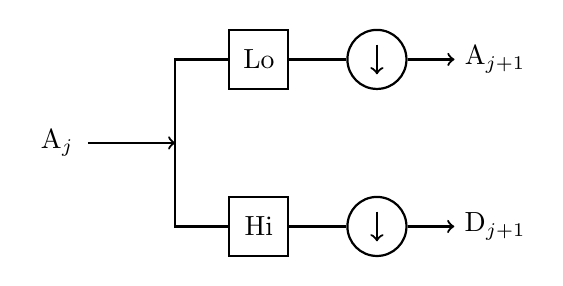
\begin{tikzpicture}[auto, node distance=1.5cm, thick, main node/.style={circle, draw}, LoHi/.style={rectangle, draw}, minimum size=.75cm]
    \node[draw=none](Aj){A$_j$};
    \node[draw=none](j1)[right of=Aj]{};
    \node[LoHi](Lo)[above right of=j1]{Lo};
    \node[LoHi](Hi)[below right of=j1]{Hi};
    \node[main node](1)[right of=Lo]{};
    \node[main node](2)[right of=Hi]{};
    \node[draw=none](Aj+1)[right of=1]{A$_{j+1}$};
    \node[draw=none](Dj+1)[right of=2]{D$_{j+1}$};

\foreach \s/\t in {Aj/j1.center, 1/Aj+1, 2/Dj+1}{
    \draw[->] (\s) -- (\t);}
\foreach \s/\t in {j1.center/Lo, j1.center/Hi}{
    \draw[](\s) |- (\t);}
\foreach \s/\t in {Lo/1, Hi/2}{
    \draw[](\s) -- (\t);}
\foreach \s in {1, 2}{
    \draw[->, shorten >=.2cm, shorten <=.2cm] (\s.north) -- (\s.south);}
\end{tikzpicture}

%\vspace{2cm}
%In the following pictures, the designation `j' stands for junction

%\begin{tikzpicture}[auto, node distance=1.5cm, thick, main node/.style={circle, draw}, LoHi/.style={rectangle, draw}, minimum size=.75cm]
%% Initial Node   	
%   \node[draw=none](LLj){LL$_j$};
%% Upper branch
%   \node[draw=none](j1)[right of=LLj]{};
%   \node[LoHi](Lo1)[above right of=j1]{Lo};
%   \node[main node](1)[right of=Lo1]{};
%   \node[draw=none](j2)[right of=1]{};
%   \node[LoHi](Hi2)[right of = j2]{Hi};
%   \node[LoHi](Lo2)[above of=Hi2]{Lo};
%   \node[main node](2)[right of=Lo2]{};
%   \node[main node](3)[right of=Hi2]{};
%   \node[draw=none](LLj+1)[right of=2]{LL$_{j+1}$};
%   \node[draw=none](LHj+1)[right of=3]{LH$_{j+1}$};
%% Lower branch
%   \node[LoHi](Hi1)[below right of=j1]{Hi};
%   \node[main node](15)[right of=Hi1]{};
%   \node[draw=none](j25)[right of=15]{};
%   \node[LoHi](Lo25)[right of = j25]{Lo};
%   \node[LoHi](Hi25)[below of=Lo25]{Hi};
%   \node[main node](25)[right of=Lo25]{};
%   \node[main node](35)[right of=Hi25]{};
%   \node[draw=none](HLj+1)[right of=25]{HL$_{j+1}$};
%   \node[draw=none](HHj+1)[right of=35]{HH$_{j+1}$};
%% Enable the labeling of Rows and Columns
%\node[draw=none, node distance=2.5cm](reference)[above of=j2]{};
%\node[draw=none, node distance=2.2cm](Rows)[left of=reference]{rows};
%\node[draw=none, node distance=2.2cm](Columns)[right of=reference]{columns};
%% Straight Edges
%\foreach \s/\t in {Lo1/1, Hi1/15, 1/j2.center, 15/j25.center, j2.center/Hi2, j25.center/Lo25,Lo2/2, Hi2/3, Lo25/25, Hi25/35}{
%    \path[draw] (\s) edge (\t);}
%% Branching edges
%\foreach \s/\t in {j1.center/Lo1, j1.center/Hi1, j2.center/Lo2, j25.center/Hi25}{
%    \draw[] (\s) |- (\t);}
%% Arrow Edges
%\foreach \s/\t in {LLj/j1.center, 2/LLj+1, 3/LHj+1, 25/HLj+1, 35/HHj+1}{
%    \draw[->] (\s) -- (\t);}
%% Arrows in Circles
%\foreach \s in {1, 2, 3, 15, 25, 35}{
%    \draw[->, shorten >=.2cm, shorten <=.2cm] (\s.north) -- (\s.south);}
%\end{tikzpicture}

\vspace{1cm}

\begin{center}
\begin{tikzpicture}
% Key
    \node[draw=none, node distance=2.5cm](K)[below of=Aj]{Key:};
    \node[rectangle, draw, minimum size=.5cm, node distance=1cm](rect)[right of=K]{};
    \node[draw=none, node distance=1.3cm](conv)[right of=rect]{= convolve};
    \node[circle, draw, minimum size=.5cm, node distance=1cm](circ)[below of=rect]{};
    \node[draw=none, node distance=1.5cm](conv)[right of=circ]{= downsample};
    \draw[->, shorten >=.1cm, shorten <=.1cm] (circ.north) -- (circ.south);
\end{tikzpicture}
\end{center}
\caption{The one-dimensional discrete wavelet transform
implemented as a filter bank.}
\label{fig:filterbank}
\end{figure}

What is going on in this algorithm? Essentially, we are extracting the wavelet coefficients by
iteratively passing our signal through the low-pass filter $L$ and the high-pass filter $H$
(referred to collectively as a \emph{filterbank}), 
and feeding the output from the low-pass filter back into the filterbank. The high-pass filter
extracts wavelet coefficients corresponding to the localized high-frequency details of the input
signal (these coefficients are name $D_j$ for \emph{d}etails), and the low-pass filter extracts
a lower-frequency approximation of the input signal (these coefficients are named $A_j$ for 
\emph{a}pproximation). Note that for the Haar Wavelet, our filters are given by
\begin{align*}
L &= \begin{bmatrix}\frac{1}{\sqrt{2}} & \frac{1}{\sqrt{2}}\end{bmatrix}\\
H &= \begin{bmatrix}-\frac{1}{\sqrt{2}} & \frac{1}{\sqrt{2}}\end{bmatrix}.
\end{align*}

As noted earlier, the key mathematical operations are convolution and down-sampling.
We now explore how to do these in Python. To accomplish the convolution, we simply use
a function in SciPy.
\begin{lstlisting}
>>> import numpy as np
>>> from scipy.signal import fftconvolve
>>> # initialize the filters
>>> L = np.ones(2)/np.sqrt(2)
>>> H = np.array([-1,1])/np.sqrt(2)
>>> # initialize a signal X
>>> X = np.sin(np.linspace(0,2*np.pi,16))
>>> # convolve X with L
>>> fftconvolve(X,L)
[ -1.84945741e-16   2.87606238e-01   8.13088984e-01   1.19798126e+00
   1.37573169e+00   1.31560561e+00   1.02799937e+00   5.62642704e-01
   7.87132986e-16  -5.62642704e-01  -1.02799937e+00  -1.31560561e+00
  -1.37573169e+00  -1.19798126e+00  -8.13088984e-01  -2.87606238e-01
  -1.84945741e-16]
\end{lstlisting}
Down-sampling is just as easy. In particular, we will down-sample by a factor
of two, which means keeping only every other entry:
\begin{lstlisting}
>>> # down-sample an array X
>>> sampled = X[1::2]
\end{lstlisting}
Putting these two operations together, we can obtain the approximation coefficients in one 
line of code:
\begin{lstlisting}
>>> A = fft.convolve(X,L)[1::2]
\end{lstlisting}
Computing the detail coefficients is done in exactly the same way, replacing $L$ with $H$.
\begin{problem}
Write a function that calculates the discrete wavelet transform as described above.
The output should be a list of one-dimensional NumPy arrays in the
following form: $[A_n, D_n, \ldots, D_1]$.
\end{problem}
% 10-15 minutes in?
Test your function by calculating the Haar wavelet coefficients of a noisy sine signal for $n=4$:
\begin{lstlisting}
>>> domain = np.linspace(0,4*np.pi, 1000)
>>> noise =  np.random.randn(1000)*.1
>>> noisysin = np.sin(domain) + noise
>>> coeffs = dwt(noisysin, L, H, 4)
\end{lstlisting}
Plot your results and verify that they match the plots in Figure \ref{fig:dwt1D}.

\begin{figure}
\centering
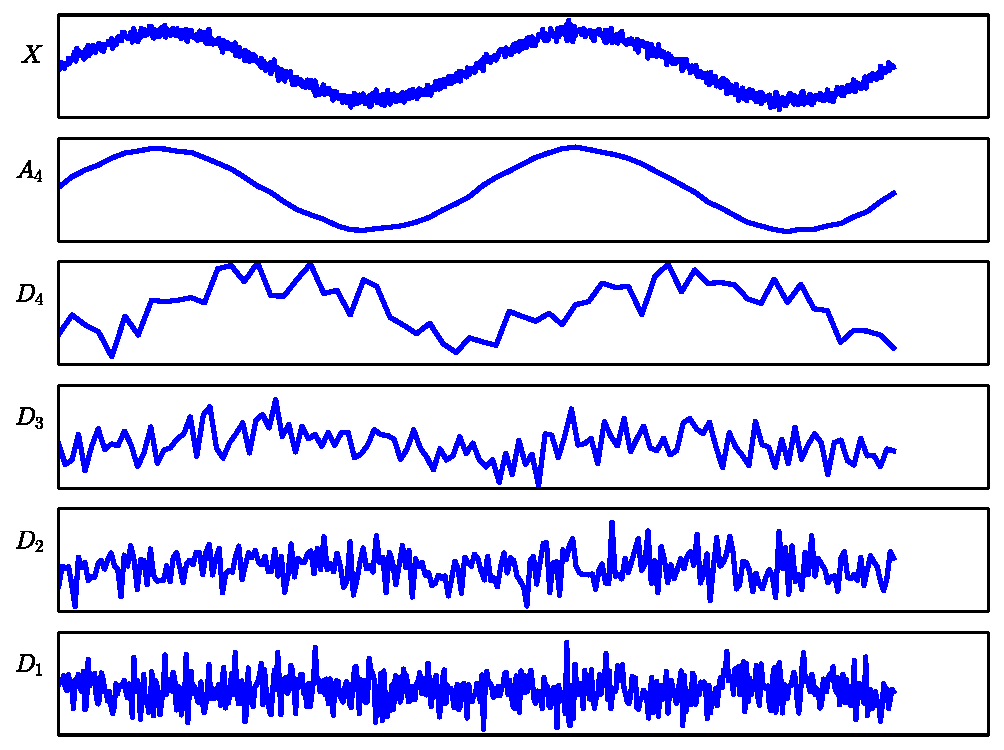
\includegraphics[width = 0.5\textwidth]{dwt1D}
\caption{A level 4 wavelet decomposition of a signal. The top panel is the original signal,
the next panel down is the approximation frame, and the remaining panels are the detail coefficients.
Notice how the approximation frame resembles a smoothed version of the original signal, while the
details capture the high-frequency oscillations and noise.}
\label{fig:dwt1D}
\end{figure}

We can now transform a one-dimensional signal into its wavelet coefficients,
but the reverse transformation is just as important. Fortunately, we can recreate a signal
from its wavelet coefficients simply by reversing the effects of the filterbank, using slightly
modified filters. The Haar wavelet filters for the inverse transformation are
\begin{align*}
L &= \begin{bmatrix}\frac{1}{\sqrt{2}} & \frac{1}{\sqrt{2}}\end{bmatrix}\\
H &= \begin{bmatrix}\frac{1}{\sqrt{2}} & -\frac{1}{\sqrt{2}}\end{bmatrix}.
\end{align*} 

Suppose we have the wavelet coefficients $A_n$ and $D_n$. Consulting Figure \ref{fig:filterbank},
we can recreate $A_{n-1}$ by tracing the schematic backwards: $A_n$ and $D_n$ are first 
\emph{up-sampled}, then they are convolved with $L$ and $H$, respectively, and finally
added together to obtain $A_{n-1}$. Up-sampling means doubling the length of an array
by inserting a 0 at every other position. In Python, this whole process looks like:
\begin{lstlisting}
>>> # up-sample the coefficient arrays A, D
>>> up_A = np.zeros(2*A.size)
>>> up_A[::2] = A
>>> up_D = np.zeros(2*D.size)
>>> up_D[::2] = D
>>> # now convolve and add, but discard last entry
>>> A = fftconvolve(up_A,L)[:-1] + fftconvolve(up_D,H)[:-1]
\end{lstlisting}
Now that we have $A_{n-1}$, we repeat the process with $A_{n-1}$ and $D_{n-1}$ to obtain
$A_{n-2}$. Proceed until we have obtained $A_0$. Since $A_0$ is defined to be the original
signal, we have finished the inverse transformation.
\begin{problem}
Write a function that calculates the inverse wavelet transform as described above.
The inputs should be a list of arrays (of the same form as the output of your discrete
wavelet transform function), the low-pass filter, and the high-pass filter. The output
should be a single array, the recovered signal. In order to check your work, compute
the discrete wavelet transform of a random array for different values of $n$, then compute the inverse
transform, and compare the original signal with the recovered signal. The difference
should be very small.
\end{problem}

\subsection*{The two-dimensional Discrete Wavelet Transform}
Our discussion so far has focused on one-dimensional
discrete signals, but it is not difficult to extend the same ideas into the
realm of two-dimensional arrays. Recall taht a digital image can be represented
as a matrix of pixel values. We can perform the wavelet decomposition of
an image in much that same way as with one-dimensional signals. We once again
calculate detail and approximation coefficients using an iterative filterbank, 
but now we generate four arrays of coefficients at each iteration as opposed to
just two. In essence, we perform the one-dimensional wavelet transform first on each
row, and then on each column of the matrix. This is quite similar to extending
the one-dimensional Fourier transform to two-dimensional images. 
We will not implement the two-dimensional discrete wavelet transform ourselves, but
instead use a Python package to be introduced presently.
See Figure \ref{fig:dwt2D} of an example of the two-dimensional Wavelet transform applied
to an image.

\begin{figure}
    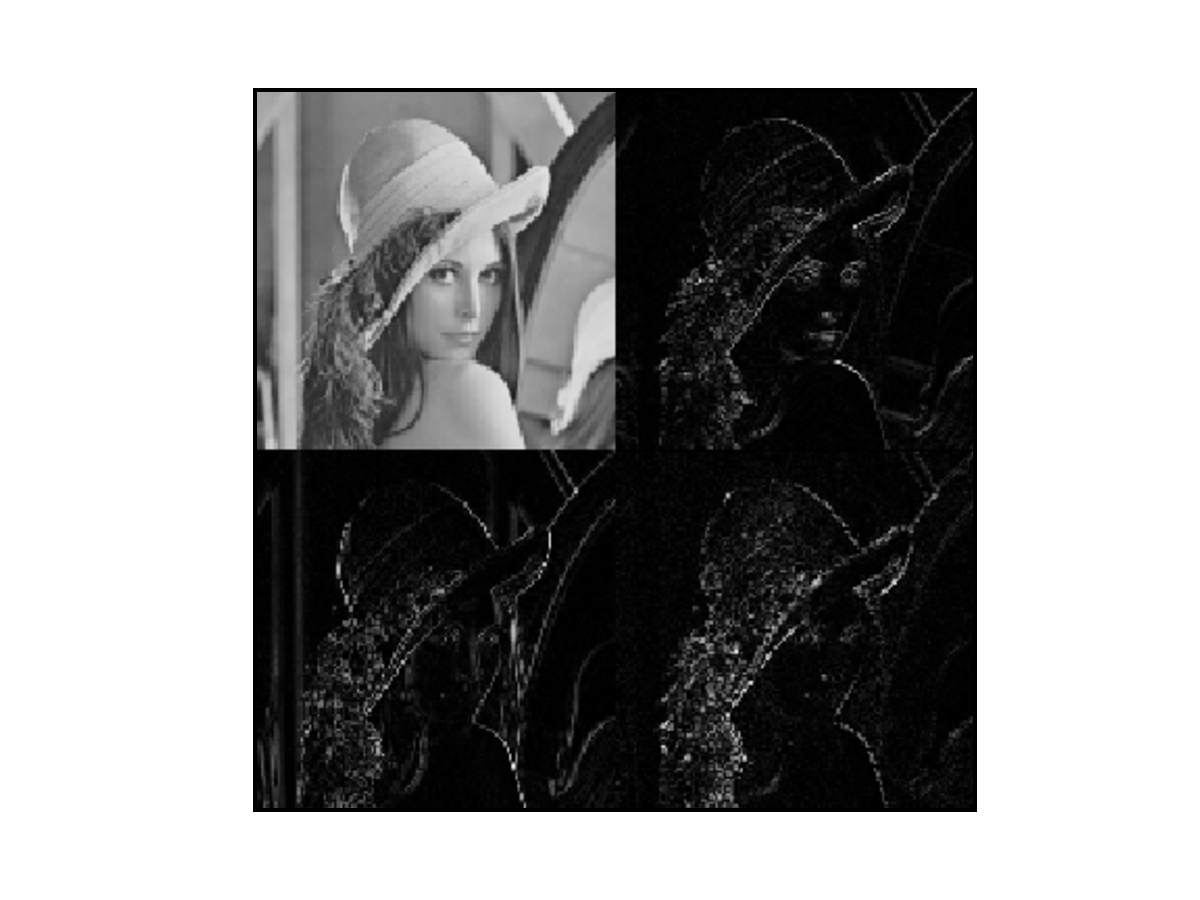
\includegraphics[width=0.8\textwidth]{dwt2D.pdf}
    \caption{The level 2 wavelet coefficients of the Lena image. The upper left quadrant
    is the approximation frame, and the other quadrants are the details. Notice how the
    details highlight the parts of the image with high-frequency textures and borders.}
    \label{fig:dwt2D}
\end{figure}

These wavelet coefficients are very useful in a variety of image processing
tasks. They allow us to analyze and manipulate images in terms of both their
frequency and spatial properties, and at differing levels of resolution.
Furthermore, wavelet bases often have the remarkable ability to represent
images in a very \textit{sparse} manner -- that is, most of the image
information is captured by a small subset of the wavelet coefficients.

\subsection*{More Wavelets}
Up to this point, the only wavelet that we have considered is the Haar wavelet,
which is the simplest example. Wavelet analysis is a broad
field, however, and there are myriad other wavelets that have been studied and
applied. See Figure \ref{fig:more_wavelets} for a couple of additional wavelets.
We will encounter more wavelets in the remainder of the lab.

\begin{figure}[H]
\minipage{0.49\textwidth}
    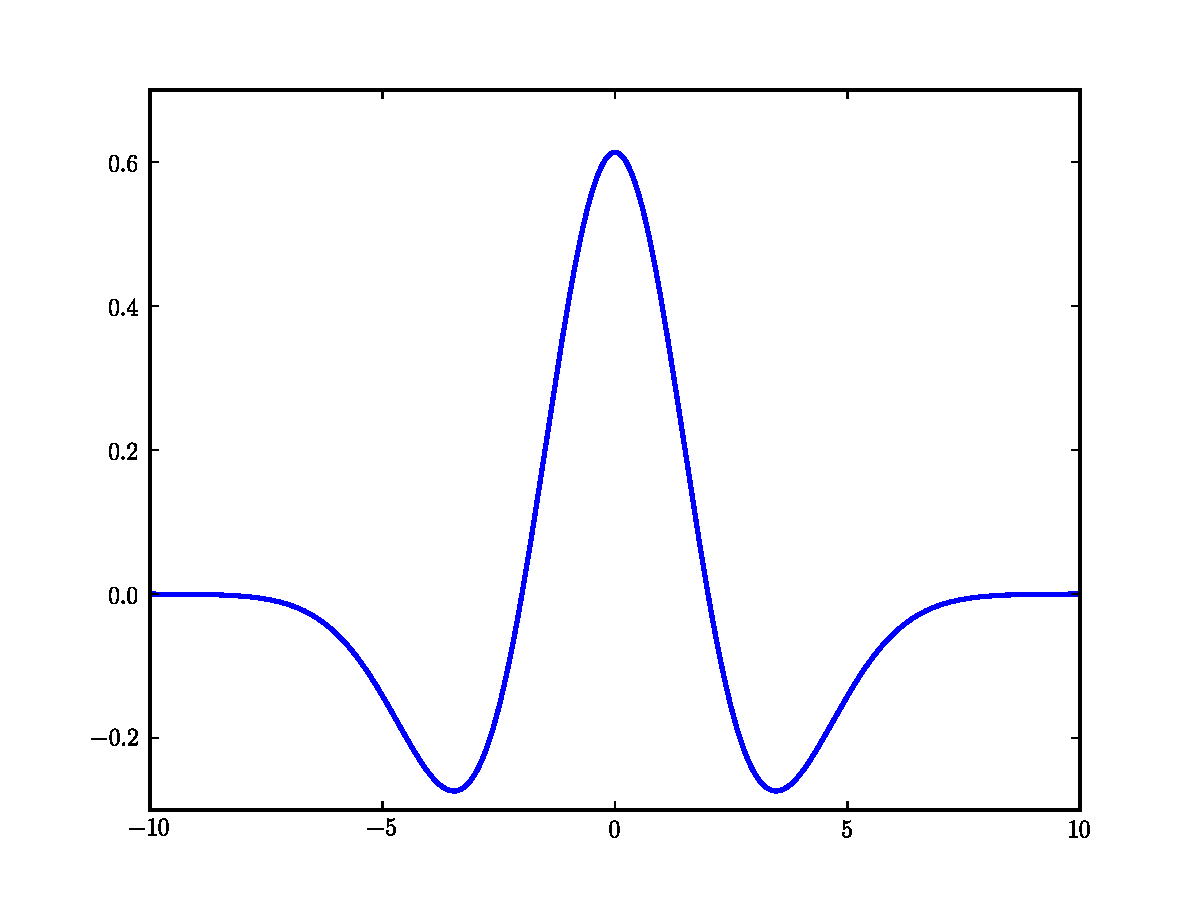
\includegraphics[width=\linewidth]{mexicanHat}
    \caption{The Mexican Hat Wavelet}
\endminipage\hfill
\minipage{0.49\textwidth}
    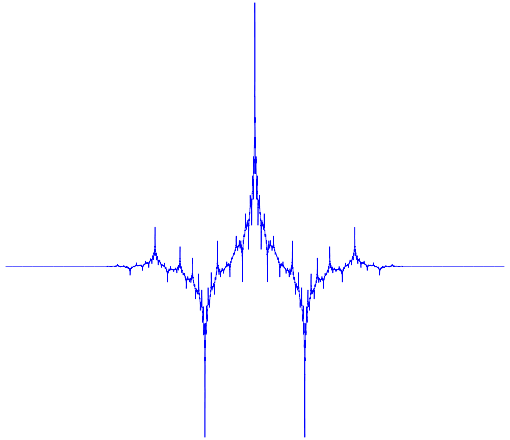
\includegraphics[width=\linewidth]{db5_3}
    \caption{The Cohen-Daubechies-Feauveau 5/3 Wavelet}
\endminipage
\label{fig:more_wavelets}
\end{figure}

\section*{The PyWavelets Module}
PyWavelets is a Python library for Wavelet Analysis. It provides convenient and
efficient methods to calculate the one and two-dimensional discrete Wavelet
transform, as well as much more. Assuming that the package has been installed on
your machine, type the following to get started:
\begin{lstlisting}
>>> import pywt
\end{lstlisting}
Performing the basic discrete Wavelet transform is very simple.
Below, we compute the one-dimensional transform for a sinusoidal signal.
\begin{lstlisting}
>>> import numpy as np
>>> f = np.sin(np.linspace(0,8*np.pi, 256))
>>> fw = pywt.wavedec(f, 'haar')
\end{lstlisting}
The variable \li{fw} is now a list of arrays, starting with the final approximation
frame, followed by the various levels of detail coefficients, just like the output
of the wavelet transform function that you coded in the previous lab.
Plot the level 2 detail and verify that it resembles a blocky sinusoid.
\begin{lstlisting}
>>> from matplotlib import pyplot as plt
>>> plt.plot(fw[-2], linestyle='steps')
>>> plt.show()
\end{lstlisting}
We can give alter the arguments to the \li{wavedec} function to use different
wavelets or obtain different levels of the wavelet transform. The second
positional argument, as you will notice, is a string that gives the name of the
wavelet to be used. We first used the Haar wavelet, with which you are already
familiar. PyWavelets supports a number of different Wavelets, however, which you can
list by executing the following code:
\begin{lstlisting}
>>> # list the available Wavelet families
>>> print pywt.families()
['haar', 'db', 'sym', 'coif', 'bior', 'rbio', 'dmey']
>>> # list the available wavelets in the coif family
>>> print pywt.wavelist('coif')
['coif1', 'coif2', 'coif3', 'coif4', 'coif5']
\end{lstlisting}
We can also include optional arguments \li{mode} and \li{level} when calling the
\li{wavedec} function. Using these arguments, you can adjust the mode for dealing
with border distortion and the level of the Wavelet decomposition, respectively.

\begin{figure}[t]
    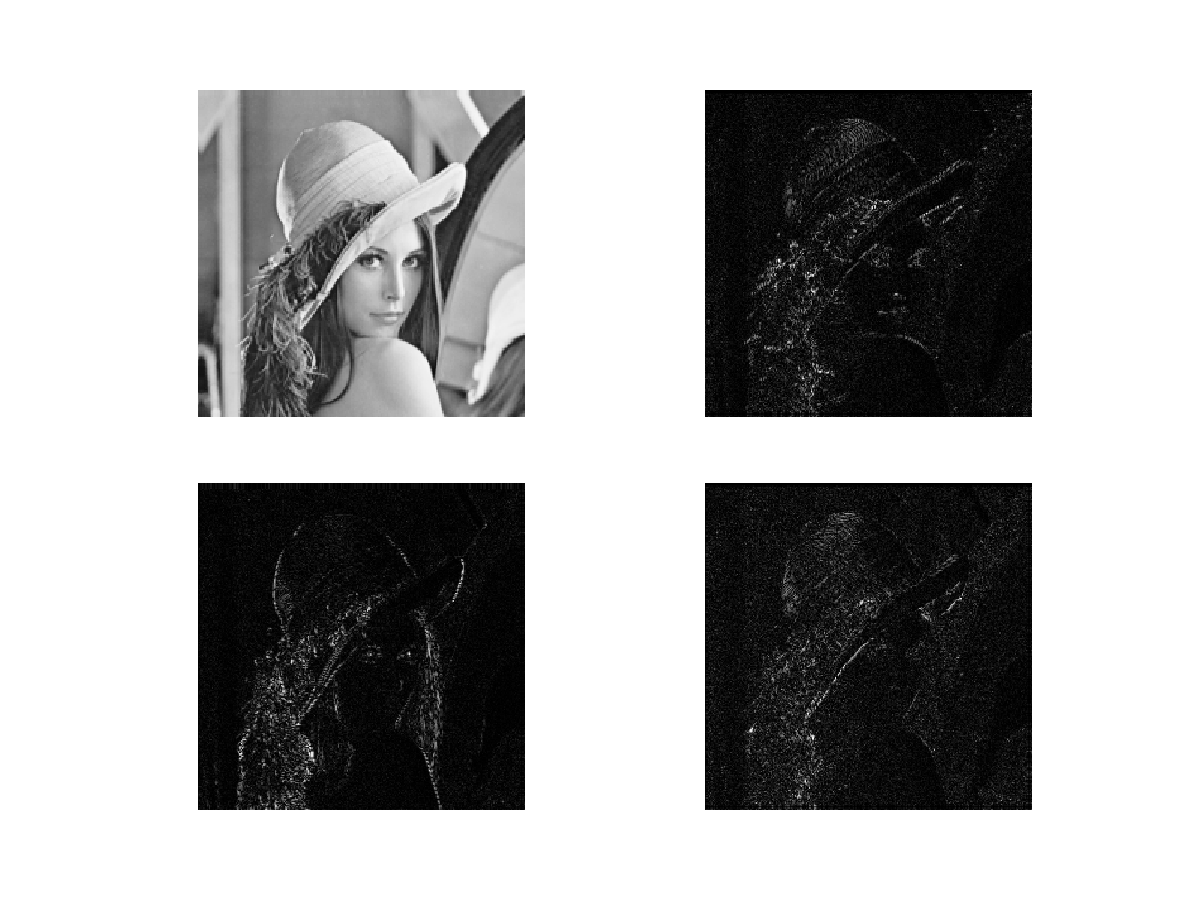
\includegraphics[width=\linewidth]{dwt2.pdf}
    \caption{Level 1 Wavelet decomposition of the Lena image.
    The upper left is the approximation frame, and the remaining
    plots are the detail coefficients.}
    \label{fig:dwt2}
\end{figure}

Now we illustrate how to perform a two-dimensional Wavelet transform using
PyWavelets. We will work with the traditional Lena image, performing a
two level wavelet transform using the Daubechies 4 Wavelet.
\begin{lstlisting}
>>> import scipy.misc
>>> lena = scipy.misc.lena()
>>> lw = pywt.wavedec2(lena, 'db4', level=2)
\end{lstlisting}
The variable \li{lw} is a list of tuples of arrays. The first entry of the list is
simply the level 2 approximation frame. The second entry of the list is a tuple of
the level 2 detail coefficients $LH$, $HL$, and $HH$ (in that order). The remaining
entries of the list are tuples containing the lower level detail coefficients.
Thus, to plot the level 1 $HL$ detail coefficients, we can execute the following code:
\begin{lstlisting}
>>> HL1 = lw[-1][1]
>>> plt.imshow(np.abs(HL1), cmap=plt.cm.Greys_r, interpolation='none')
>>> plt.show()
\end{lstlisting}
The output of this code should be a plot resembling the lower left plot given in Figure
\ref{fig:dwt2}.

We have only introduced a couple of the basic tools available in PyWavelets. There
are of course many more functions and methods that facilitate a more comprehensive
Wavelet analysis.

\begin{comment}
This section could be cool, but it's not hashed out very well yet.
\section*{Edge Detection}
It is often useful to identify the edges of objects and figures
represented in images. The edge information can be used to classify images
and group them with other similar images (this is part of a field called
\textit{computer vision}), to segment the image into component parts, to
sharpen blurry images, to filter out unnecessary details of the image,
and so forth. Of course, our human eyes are very adept at recognizing edges,
but enabling a computer to do the same is much more difficult. An edge can
be thought of as a discontinuity in the image or a region of high contrast
in either color or brightness. We can therefore leverage the high-frequency
detail coefficients of the wavelet transform to detect the edges. Execute the
following code:
\begin{lstlisting}
>>> # calculate one level of wavelet coefficients
>>> coeffs = pywt.wavedec2(lena,'haar', level=1)
\end{lstlisting}

Note that the approximation coefficients are very close to the original
image, while the detail coefficients are much more sparse, and roughly
capture the edges in the image. In particular, the upper right coefficients
emphasize the vertical edges, the lower left coefficients emphasize the
horizontal edges, and the lower right coefficients emphasize the diagonal
edges.

\begin{problem}
Now zero out the approximation coefficients and use your inverse DWT
function to recreate the image. Plot its absolute value. This image is
a fairly good representation of the edges. If we add this to the original
image, we can increase the contrast at the edges (that is, make the dark
side darker, and the light side lighter). Do this, and plot the original
image side-by-side with the sharpened image. What do you notice? There
are many image-sharpening techniques, and those based on wavelets
are more sophisticated than what we have done here, but this gives the
basic idea.
\end{problem}
the above section needs work, or maybe should be taken out completely.
\end{comment}

\begin{comment}
This section is good, but there's just not room for it in this lab if we
want a fairly complete section on image compression.
\section*{Noise Removal}
Noise in an image can be defined as unwanted visual artifacts that
obscure the true image. Images can acquire noise from a variety of
sources, including the camera, transmission, and image processing
algorithms. Noise can be completely random and incoherent (as in
Figure \ref{fig:incoherent}), or it can be coherent and display
visual patterns (Figure \ref{fig:coherent}). In this section, we will
focus on reducing a particular type of random noise in images, called
\textit{Gaussian white noise}.

\begin{figure}[t]
\minipage{0.49\textwidth}
    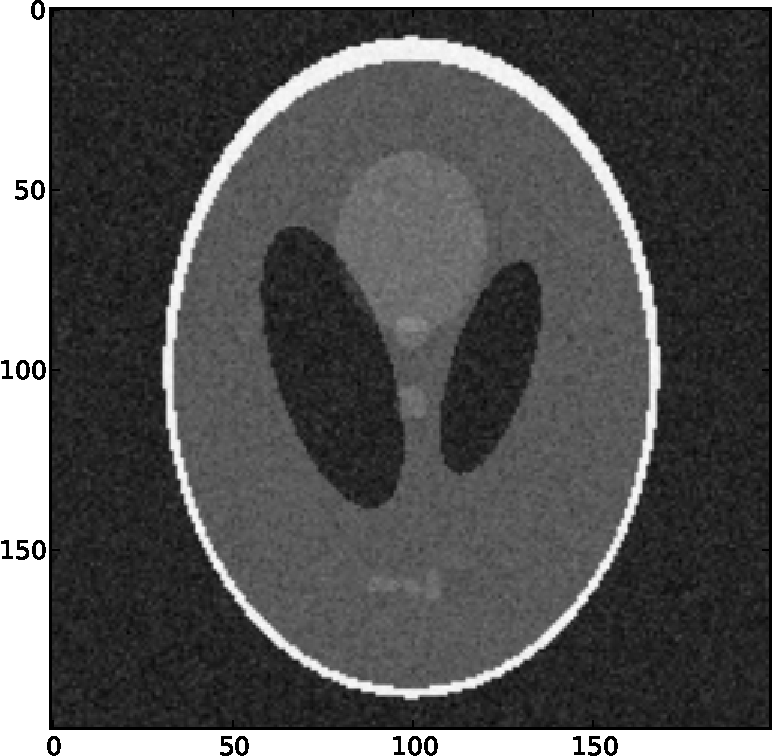
\includegraphics[width=\linewidth]{phantom_random.pdf}
    \caption{The Phantom image with incoherent noise}
    \label{fig:incoherent}
\endminipage\hfill
\minipage{0.49\textwidth}
    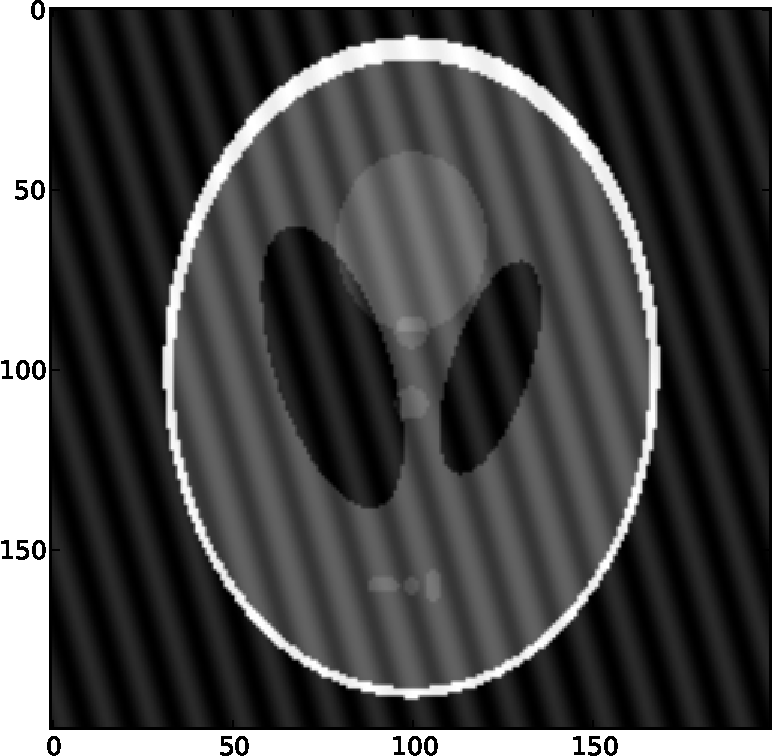
\includegraphics[width=\linewidth]{phantom_coherent.pdf}
    \caption{The Phantom image with coherent noise}
    \label{fig:coherent}
\endminipage
\end{figure}

An image that is distorted by Gaussian white noise is one in which
every pixel has been perturbed by a small amount, such that the
perturbations are normally distributed. We can easily add such noise
to an image using the \li{np.random.normal} function.

\begin{lstlisting}
>>> noisyLena = lena + np.random.normal(scale=20, size=lena.shape)
>>> plt.imshow(noisyLena, cmap=plt.cm.Greys_r)
>>> plt.show()
\end{lstlisting}

Given an image with Gaussian white noise, how do we go about reducing
the noise level? Our approach will be based on the idea of thresholding.
It turns out that images are often sparse in the wavelet basis,
particularly in the high-frequency details. The Gaussian noise, however,
is very high frequency, and thus its wavelet transform will be
concentrated in high-frequency wavelet coefficients (of magnitude
roughly proportional to the variance of the noise). We can therefore
reduce the noise while preserving the true image by shrinking the
detail coefficients via hard or soft thresholding.

Given a positive threshold value $\tau$, hard thresholding sets
every wavelet coefficient whose magnitude is less than $\tau$ to
zero, while leaving the remaining coefficients untouched. Soft
thresholding also zeros out all coefficients of magnitude less than
$\tau$, but in addition maps every other coefficient $\beta$ to
$\beta - \tau$ if $\beta > 0$ or $\beta + \tau$ if $\beta < 0$.

Implementing these simple thresholding algorithms in Python is
straight-forward, but PyWavelets already provides this functionality.
The following code gives an example.

\begin{lstlisting}
>>> A = np.arange(-4,5).reshape(3,3)
>>> A
array([[-4, -3, -2],
       [-1,  0,  1],
       [ 2,  3,  4]])
>>> pywt.thresholding.hard(A,1.5)
array([[-4, -3, -2],
       [ 0,  0,  0],
       [ 2,  3,  4]])
>>> pywt.thresholding.soft(A,1.5)
array([[-2.5, -1.5, -0.5],
       [ 0. ,  0. ,  0. ],
       [ 0.5,  1.5,  2.5]])
\end{lstlisting}

Once the coefficients have been thresholded, we take the inverse
wavelet transform to recover the denoised image. This can be done
by calling the \li{waverec2} function, providing the list of Wavelet
coefficients as well as the name of the desired Wavelet as arguments.
The threshold value is generally a function of the variance of the noise,
and in real situations, we do not know what this variance is. In fact,
noise variance estimation in images is a research area in its own
right, but this goes beyond the scope of this lab, and so we will
assume that we already have a decent estimate of the variance.

\begin{figure}[t]
    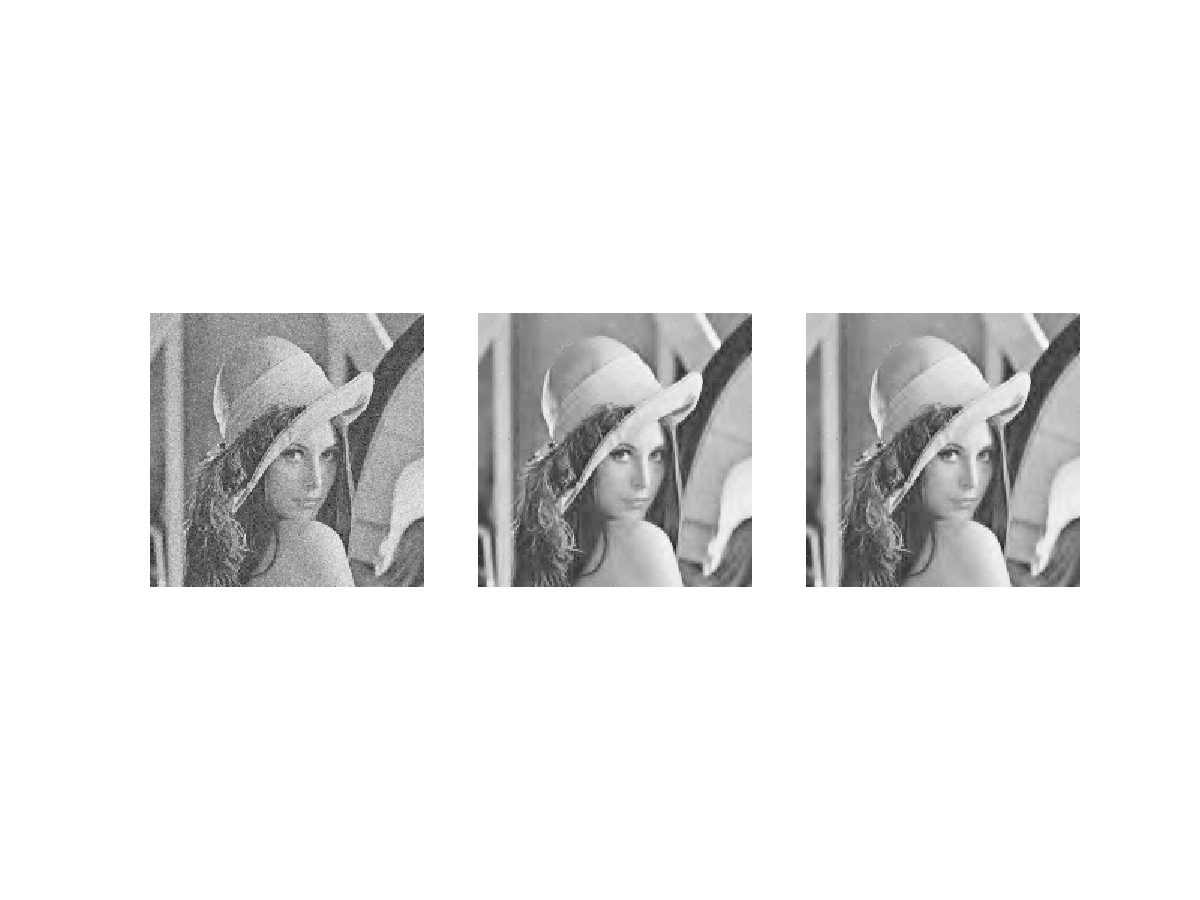
\includegraphics[width=\linewidth]{denoise.pdf}
    \caption{Noisy Lena (left), denoised using hard thresholding (center),
    and denoised using soft thresholding (right).}
    \label{fig:denoise}
\end{figure}

\begin{problem}
Write functions that implement the hard and soft thresholding
techniques. The inputs should be a list of wavelet coefficients
in the usual form, as well as the threshold value. The output
should be the thresholded wavelet coefficients (also in
the usual form). Remember that we only want to threshold the
detail coefficients, and not the approximation coefficients.
You should therefore leave the first entry of the input
coefficient list unchanged.
\end{problem}

\begin{problem}
Create a noisy version of the Lena image by adding Gaussian
white noise of mean 0 and standard deviation $\sigma = 20$ (i.e. \li{scale=20}).
Compute four levels of the wavelet coefficients using the Daubechies 4 Wavelet,
and input these into your
thresholding functions (with $\tau = 3\sigma$ for the hard threshold,
and $\tau = 3\sigma/2$ for the soft threshold). Reconstruct the
two denoised images, and then plot these together alongside the
noisy image. Your output should match Figure \ref{fig:denoise}.

What do you notice? How does lowering or raising the
threshold affect the reconstructed images? What happens if you use
a different Wavelet?
\end{problem}
\end{comment}


\section*{Image Compression}
We now turn to the topic of image compression.
Numerous image compression techniques
have been developed over the years seeking to reduce the cost of storing large quantities of images.
Transform methods, which utilize transformations such as the Fourier or Wavelet transforms,
have long played an important role in these techniques;
for example, the popular JPEG image compression standard is based on
the discrete cosine transform. Starting from the early 1990s, much
research has gone into compression methods using the discrete wavelet
transform, and to great success. The JPEG2000 compression standard
and the FBI Fingerprint Image database, along with other systems,
take the wavelet approach.

The general framework for compression is fairly straightforward. First,
the image to be compressed undergoes some form of preprocessing (this
can include subtracting out its mean, tiling the image, or perhaps
nothing at all). Next, the discrete wavelet transform is used to calculate
the wavelet coefficients, and these are then \textit{quantized},
i.e. mapped to a set of discrete values. The quantized coefficients are
then passed through an entropy encoder, which reduces
the number of bits required to store the coefficients.
What remains is a compact stream of bits
that can then be saved or transmitted much more efficiently than the
original image. All of the above steps are invertible, allowing us to
reconstruct the image from the compressed bitstream. See Diagram
\ref{tikz:wsqscheme}.

\begin{figure}
\centering
\begin{tikzpicture}[rect/.style= {draw=none, node distance = 3cm},
	rect2/.style = {draw, thick, minimum width=3cm, minimum
	height=1cm}, >=stealth', shorten >=2pt]

\node[rect] (IM) [] {Image};
\node[rect2, node distance=3cm] (PR) [right of = IM]
	{Pre-Processing};
\node[rect2, node distance=4.5cm] (WD)[right of= PR]
	{Wavelet Decomposition};
\node[rect2, node distance=1.75cm](Q) [below=of PR.west, anchor=west]
	{Quantization};
\node[rect2, node distance = 1.75cm](EC)[below=of WD.west, anchor=west]
	{Entropy Coding};
\node[rect, node distance= 3.5cm](BS)[right of=EC]
	{Bit Stream};

\foreach \s/\t in {IM/PR, PR/WD, Q/EC, EC/BS}
	{\path[->, thick](\s) edge (\t);}
\draw[|-,-|,->, thick](WD.south) |-+(0,-1em)-| (Q.north);


\end{tikzpicture}
\caption{Wavelet Image Compression Schematic}
\label{tikz:wsqscheme}
\end{figure}

\subsection*{WSQ: The FBI Fingerprint Image Compression Algorithm}
The Wavelet Scalar Quantization (WSQ) algorithm is among the first successful wavelet-based image compression algorithms.
It solves the problem of storing millions of fingerprint scans efficiently while meeting the law enforcement requirements for high image quality.
This algorithm is capable of achieving compression ratios in excess of 10-to-1 while retaining excellent image quality.
See Figure \ref{fig:finger_compression}.
We will implement a basic version of this algorithm.

\begin{figure}
\centering
\begin{subfigure}{.32\textwidth}
  \centering
  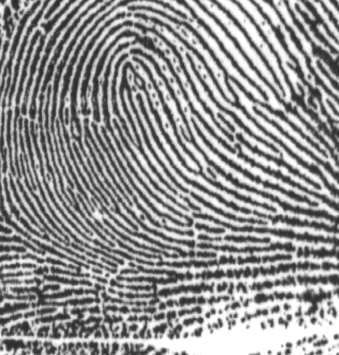
\includegraphics[width=.7\linewidth]{uncompressed_finger.png}
  \caption{Uncompressed}
  \label{fig:sub1}
\end{subfigure}%
\begin{subfigure}{.32\textwidth}
  \centering
  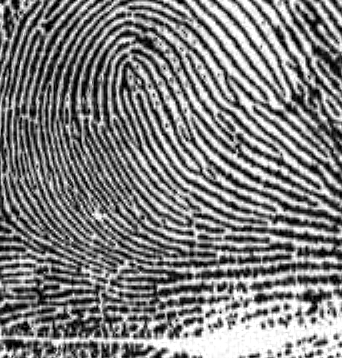
\includegraphics[width=.7\linewidth]{compressed_finger(30comp).png}
  \caption{30:1 compressed}
  \label{fig:sub1}
\end{subfigure}%
\begin{subfigure}{.32\textwidth}
  \centering
  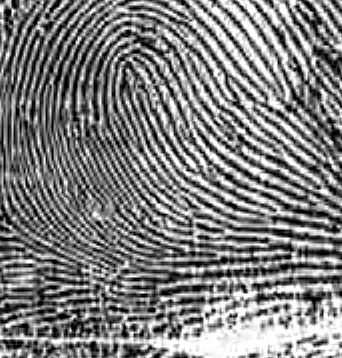
\includegraphics[width=.7\linewidth]{compressed_finger(60comp).png}
  \caption{60:1 compressed}
  \label{fig:sub2}
\end{subfigure}
\caption{Fingerprint scan at different levels of compression.}
\label{fig:finger_compression}
\end{figure}

\subsection*{WSQ: Preprocessing}
The input to the algorithm is a matrix of nonnegative 8-bit integer values giving
the grayscale pixel values for the fingerprint image. We process the image
by the following formula:
\[
M' = \frac{M-m}{r},
\]
where $M$ is the original image matrix, $M'$ is the processed image,
$m$ is the mean pixel value, and $r = \max\{\max(M) - m, m - \min(M)\}/128$
(here $\max(M)$ and $\min(M)$ refer to the maximum and minimum pixel values
in the matrix). This preprocessing serves to ensure that roughly half of the
new pixel values are negative, while the other half are positive, and all fall
in the range $[-128,\,128]$.
\begin{problem}
Implement the preprocessing step, as well as its inverse. Note that to invert
the pre-processing, you will need to know the values for $m$ and $r$. Hence,
these values need to persist over the course of the entire algorithm.
\end{problem}

\subsection*{WSQ: Calculating the Wavelet Coefficients}
The official standard for the WSQ algorithm uses a slight modification of the
discrete wavelet transform that we have studied in this lab. The differences
are somewhat technical and do not affect performance drastically, so we will
stick with the PyWavelets implementation.

INSERT SUBBAND PATTERN DIAGRAM (USE TIKZ GRID)

We need to calculate the subband pattern found in Diagram REFERENCE.
While this pattern may appear complicated at first, we can obtain the
required subband coefficients rather easily. To start, decompose the image
into 16 subbands, first by using the \li{dwt2} function to split the
image into four subbands, and then applying the function again to each of the
four subbands. You may find it helpful to write a function that accomplishes
just this task. You should now have a grid of 16 subbands.

Next, split each of the three subbands found in the top left corner of the subband
grid into 16 additional subbands, in the same way as before. You now have a grid
of $13 + 3(16) = 61$ subbands.

Finally, take the very top left subband, and split this into four additional subbands.
You should have 64 subbands. Place them into a list in the order indicated by
the number in Diagram REFERENCE.

\begin{problem}
Implement the subband decomposition as described above. The input is a matrix
and the output is a list of the 64 subbands in the order indicated.

Implement the inverse of this decomposition, i.e. write code that will take
a list of the 64 subbands and reproduce the original matrix. Your code will
need to make use of the \li{idwt2} function to compute the inverse discrete
wavelet transform.
\end{problem}

\subsection*{WSQ: Quantization}
By quantization, we mean the process of mapping each wavelet coefficient to an
integer value. Quantization is the main source of compression in the algorithm. By mapping
the wavelet coefficients to a relatively small set of integer values, we reduce
the complexity of the data, which will allow us to efficiently encode the information
in a bit string. Further, a large portion of the wavelet coefficients will be mapped to 0
and discarded completely. We must take care, however, to perform this quantization in a
manner that achieves good compression without discarding so much information that we
are unable to reconstruct the image accurately.

Given a wavelet coefficient $a$ in subband $k$, the corresponding quantized
coefficient $p$ is given by
\[
p =
\begin{cases}
   \left\lfloor\frac{a-Z_k/2}{Q_k}\right\rfloor + 1, & a> Z_k/2 \\
   0,       & -Z_k/2 \leq a \leq Z_k/2\\
   \left\lceil\frac{a + Z_k/2}{Q_k}\right\rceil - 1, & a < -Z_k/2
  \end{cases}
\]
The values $Z_k$ and $Q_k$ are dependent on the subband, and determine how much
compression is achieved. If $Q_k=0$, we simply map the coefficient to 0.
Selecting appropriate values for these parameters is a
tricky problem in itself, so we provide you with a list of these values for each
subband.

Note that quantization is not a perfectly invertible process. Once we have quantized
the wavelet coefficients, some information is permanently lost. However, we can
roughly reconstruct the wavelet coefficients from the quantized coefficients
using the following formula (where again, this is for a quantized coefficient $q$
in subband $k$, and $\hat{a}_k$ refers to the reconstructed wavelet coefficient).
This process is called \emph{dequantization}.
\[
\hat{a}_k =
\begin{cases}
(p-C)Q_k + Z_k/2, & p> 0\\
0, & p = 0\\
(p + C)Q_k - Z_k/2, & p < 0
\end{cases}
\]
For our purposes, take $C = 0.44$.
\begin{problem}
Implement the quantization step. The inputs should be a list of the 64 subbands, as
well as a list containing the parameter values $Z_k$ and $Q_k$ for each of the 64
subbands. The output should be a list of the 64 quantized subbands. Try to use
vectorization to simplify the coding and increase efficiency.

Implement the dequantization step as well. The inputs to this step should be
a list of the 64 quantized subbands, as well as the list of parameter values
for each subband. The output should be a list of the 64 subbands containing
the reconstructed wavelet coefficients.
\end{problem}
\subsection*{WSQ: Grouping}
At this point in the algorithm, you should have a list of length 64, where the $k$-th
entry is a matrix containing the quantized wavelet coefficients for the $k$-th subband.
We will segment this list into three groups, each group containing the quantized coefficients
for a particular subset of subbands. The effect of this grouping to that we obtain three
lists of quantized coefficients, and each of these lists has a higher degree of homogeneity
than the original list of all 64 quantized subbands. This is important for the entropy coding,
since we can achieve better compression when encoding groups of similar coefficients separately.

Group subbands $0$ through $18$ together, $19$ through $51$ together, and finally $52$ through $63$
together. You may understand the logic of these groupings when glancing back at Diagram REFERENCE.
Each group should be a list of numbers rather than matrices. Below is sample code for producing the
first group. You a similar approach for forming the other two groups.
\begin{lstlisting}
>>> # assume coeffs is my list of the 64 quantized subbands
>>> group1 = []     # this will hold the group 1 coefficients
>>> shapes1 = []    # this keeps track of the subband dimensions
>>> for i in xrange(19):
>>>     shapes1.append(coeffs[i].shape)
>>>     group1.extend(coeffs[i].ravel())
\end{lstlisting}
Notice that the code also produces a list containing the dimensions of each of the subbands in the group.
This is useful when recreating the subbands from the list of coefficients. We can do this
reconstruction for the first group as follows:
\begin{lstlisting}
>>> # reconstruct the subbands from the group1 values
>>> new_coeffs = []     # this will hold the reconstructed subbands
>>> i = 0
>>> for shape in shapes1:
>>>     l = shape[0]*shape[1] # number of entries in the subband
>>>     new_coeffs.append(np.array(group1[i:i+l]).reshape(shape))
\end{lstlisting}
\begin{problem}
Implement the grouping procedure and its inverse, as described above. You will need to
keep track of the lists containing the dimensions of the subbands over the course
of the algorithm, as these are needed in the reconstruction phase.
\end{problem}
\subsection*{Reading and Writing Bits with bitstring}
In the final stage of the algorithm, we take our groups of quantized coefficients
and map them to bit patterns. We then concatenate these bit patterns into a single
bit string, and write this to file. Pure Python is not equipped to manipulate data
at the bit level, so we will use the Python package \li{bitstring} to facilitate
the process. In this section we work through a quick tutorial on \li{bitstring}
that will present the functions required for the WSQ algorithm.

Once you have installed the package, type the import command:
\begin{lstlisting}
>>> import bitstring as bs
\end{lstlisting}
In order to build a string of bits, we initialize a \li{BitArray} object, and then add the
desired bit patterns.
\begin{lstlisting}
>>> bits = bs.BitArray()
>>> bits.append('0b1101')
>>> bits.append('0b01')
\end{lstlisting}
We can add an 8- or 16-bit representations of an integer as follows:
\begin{lstlisting}
>>> # add the 8-bit integer 212, and then the 16-bit integer 1047
>>> bits.append('uint:8=212')
>>> bits.append('uint:16=1047')
\end{lstlisting}
To view the bits contained in the \li{BitArray}, we can print the \li{bin} attribute.
To save the bits to file, we can call the \li{tofile()} method.
\begin{lstlisting}
>>> # view the entire bit string
>>> print bits.bin
110101110101000000010000010111

>>> # save to file
>>> f = file('bits.bs', 'wb')
>>> bits.tofile(f)
>>> f.close()
\end{lstlisting}

Now let's read the bits in the file. Since we will only be reading, and not altering,
the bit stream in the file, we will use a \li{ConstBitStream} object.
\begin{lstlisting}
>>> bitreader = bs.ConstBitStream(filename='bits.bs')
>>> # check to see how many bits are in the stream
>>> print bitreader.length
32
\end{lstlisting}
Notice that the length of the bit stream in the file is 32, whereas we only wrote 30 bits to file.
The reason for this is that a file must contain byte-sized chunks of data. Since a byte is 8 bits,
the \li{bitstring} package automatically appends enough 0 bits when writing the bit stream so that
its length is a multiple of 8.

When reading the data from a bit stream, we simply call the \li{read} method, giving it an input string
that specifies the way to interpret the bits, and the number of bits to read. To read the next 3 bits as
binary, the input string would be \li{'bin:3'}, whereas to read the next 16 bits as an unsigned integer
you would provide the input string \li{'uint:16'}.
Let's read the first 6 bits, one at a time:
\begin{lstlisting}
>>> for i in xrange(6):
>>>     print bitreader.read('bin:1')
1
1
0
1
0
1
\end{lstlisting}
We know that the next 8 bits should be interpreted as an unsigned integer, and likewise for the
following 16 bits. Thus, we read these bits as follows:
\begin{lstlisting}
>>> print bitreader.read('uint:8')
212
>>> print bitreader.read('uint:16')
1047
\end{lstlisting}
The final two bits, as explained above, are simply zeros that were added for file alignment purposes:
\begin{lstlisting}
>>> print bitreader.read('bin:2')
00
\end{lstlisting}
You now have all the tools necessary to read and write the compressed image bit stream.

\subsection*{WSQ: Huffman Coding}
Huffman coding is a technique for assigning binary codes to a collection of symbols in such a way
that minimizes the total number of bits needed to encode the symbols.
More frequent symbols will be assigned shorter binary codes, while rare symbols will have
longer codes. Although it is not difficult to calculate the Huffman codes for a given collection
of symbols, in this lab we will assume that the codes have already been generated and given to
us. Our task lies in simply converting the quantized coefficients into their correct binary codes.

The WSQ standard instructs us to generate Huffman codes separately for each of the three groups
of quantized coefficients, and so we provide you with three lists containing these codes.

 The step in this process that we will focus on is quantization. Put simply,
 quantization is a process whereby the coefficients are converted into
 integers. If the coefficients are floating-point numbers, then this
 process introduces some loss of precision, and we call this \textit{
 lossy compression}. In the situation where all the coefficients are already
 integers, it is possible to compress the image without any loss of precision,
 and this is called \textit{lossless compression}. Quantization can be
 performed in a variety of ways, and we will explore one particular method
 called a \emph{uniform null-zone quantizer}. Given a coefficient $x$, we assign
 to it an integer $q$ given by
\begin{equation*}
q =
 \begin{cases}
   \lceil x / \delta - t/2 \rceil, &  x \geq 0\\
   \lfloor x / \delta + t/2 \rfloor & x \leq 0
 \end{cases}
\end{equation*}
where $1 \leq t \leq 2$ and $\delta > 0$ are adjustable parameters.
The inverse process, called de-quantization, consists of recovering
the coefficient $y$ from the quantized value $q$ via the equation
\begin{equation*}
 y =
  \begin{cases}
   (q - 1/2 + t/2)\delta & q > 0\\
   (q + 1/2 - t/2)\delta & q < 0\\
   0,                    & q = 0
  \end{cases}
 \end{equation*}
What we are essentially doing is mapping all wavelet coefficients that
fall in the interval $[-\delta,\delta]$ to 0 and all wavelet coefficients
in the interval $[j\delta,(j+1)\delta]$ to $(2j+1)\delta/2$ for integers
$j \geq 1$ and $j \leq -2$. This greatly reduces the number of distinct
coefficient values (indeed, most of the coefficients are mapped to
zero), allowing us, at the cost of some precision, to store less
information. The larger we choose $\delta$, the more compression we
can achieve, albeit with a correspondingly larger loss in precision.
\begin{problem}
Write function \li{quantize} and \li{dequantize} based on the discussion above.
In both cases, the inputs should be a list of wavelet coefficients in
standard form, the $\delta$ parameter, and the $t$ parameter with default
value of 2. The functions should return the quantized list of wavelet
coefficients.

For the Lena image, calculate the complete set of wavelet coefficients and then
quantize and de-quantize the coefficients, and reconstruct the image.
Do this for a few different values of $\delta$ (with $t=2$), and observe how
the image is distorted. Try using different Wavelets. Keep in mind that there are
specially designed Wavelets used in image compression that are not available
in PyWavelets, so distortion will be greater than tolerable in real-life settings.
\end{problem}


\begin{comment}
We don't need a lot of this expository content in the lab.
\subsection*{The Haar Wavelet}

As noted earlier, the Fourier transform is based on the complex exponential
function. Let us alter the situation and consider instead the following
function, known as the \emph{Haar wavelet}:
\begin{equation*}
\psi(x) =
 \begin{cases}
  1 & \text{if } 0 \leq x < \frac{1}{2} \\
  -1 & \text{if } \frac{1}{2} \leq x < 1 \\
  0 & \text{otherwise.}
 \end{cases}
\end{equation*}

% It might be nice to plot this function and include the image in the lab.

Along with this wavelet, we introduce the associated \emph{scaling function}:
\begin{equation*}
\phi(x) =
 \begin{cases}
 1 & \text{if } 0 \leq x < 1 \\
 0 & \text{otherwise.}
 \end{cases}
\end{equation*}

From the wavelet and scaling function, we can generate two countable families
of dyadic dilates and translates given by
\begin{equation*}
\psi_{m,k}(x) = \psi(2^mx - k)
\end{equation*}
\begin{equation*}
\phi_{m,k}(x) = \phi(2^mx - k),
\end{equation*}
where $m,k \in \mathbb{Z}$.

Let us focus for the moment on that second family of functions, $\{\phi_{m,k}\}$.
If we fix $m$ and let $k$ vary over the integers, we have a countable collection of
simple functions. The support of a typical function $\phi_{m,k}$ is the interval
$[k2^{-m}, (k+1)2^{-m}]$, and for any $m \in \mathbb{Z}$ we have
\begin{equation*}
\mathbb{R} = \displaystyle\biguplus_k\,[k2^{-m}, (k+1)2^{-m}],
\end{equation*}
where $\uplus$ denotes a union over disjoint sets. Thus, the supports can be viewed as
a discretization of the real line, and we can use this collection of simple functions
to approximate any $f \in L^2(\mathbb{R})$ in the following sense:
\begin{equation*}
f(x) \approx f_m(x) := \displaystyle\sum_{k \in \mathbb{Z}}\alpha_{m,k}\phi_{m,k}(x),
\end{equation*}
where
\begin{equation*}
\alpha_{m,k} := 2^m \displaystyle \int_{k2^{-m}}^{(k+1)2^{-m}}f(x) dx
\end{equation*}
($\alpha_{m,k}$ is simply the average value of $f$ on $[k2^{-m},(k+1)2^{-m}]$). As you
would probably expect, the point-wise error between $f$ and its approximation $f_m$
(called a \emph{frame}) goes to zero as $m \to \infty$.

These frames are not quite good enough, however. Each coefficient $\alpha_{m,k}$
certainly captures local information about $f$ -- namely its average value on
a certain interval -- but it fails to tell us anything about how $f$ changes
on that interval. We need more information than is provided by $f_m$ in order
to know about discontinuities or high-frequency oscillations of $f$. To this end,
we now consider the wavelet function $\psi$.
Notice that the Haar wavelet is oscillatory in nature, and is thus better suited
to capture local information on how a function changes at a given point. For
any given $m$, we define a function $d_m$, called a \emph{detail}, as follows:
\begin{equation*}
d_m(x) := \displaystyle\sum_{k \in \mathbb{Z}}\beta_{m,k}\psi_{m,k}(x),
\end{equation*}
where
\begin{equation*}
\beta_{m,k} := 2^m \displaystyle \int_{-\infty}^{\infty}f(x) \psi_{m,k}(x) dx.
\end{equation*}
Each coefficient $\beta_{m,k}$ gives information about how $f$ changes on the
the interval $[k2^{-m}, (k+1)2^{-m}]$, and larger coefficients correspond
to larger spikes of width $2^{-m}$. Thus, as $m$ increases, the
detail function $d_m$ gives information about the higher-frequency oscillations
of the function. The details and approximation frames interact in the following way:
\begin{equation*}
f_{m+1} = f_m + d_m.
\end{equation*}
As a result of this fortuitous relationship, one can prove the decomposition
\begin{equation*}
L^2(R) = V_0 \oplus W_0 \oplus W_1 \oplus \cdots,
\end{equation*}
where $V_j := \text{span}\{\phi_{j,k}\}_{k \in \mathbb{Z}}$ and
$W_j := \text{span}\{\psi_{j,k}\}_{k \in \mathbb{Z}}$. This fact justifies
our hope to approximate and analyze functions using wavelets.
\begin{figure}[t]
\minipage{0.32\textwidth}
    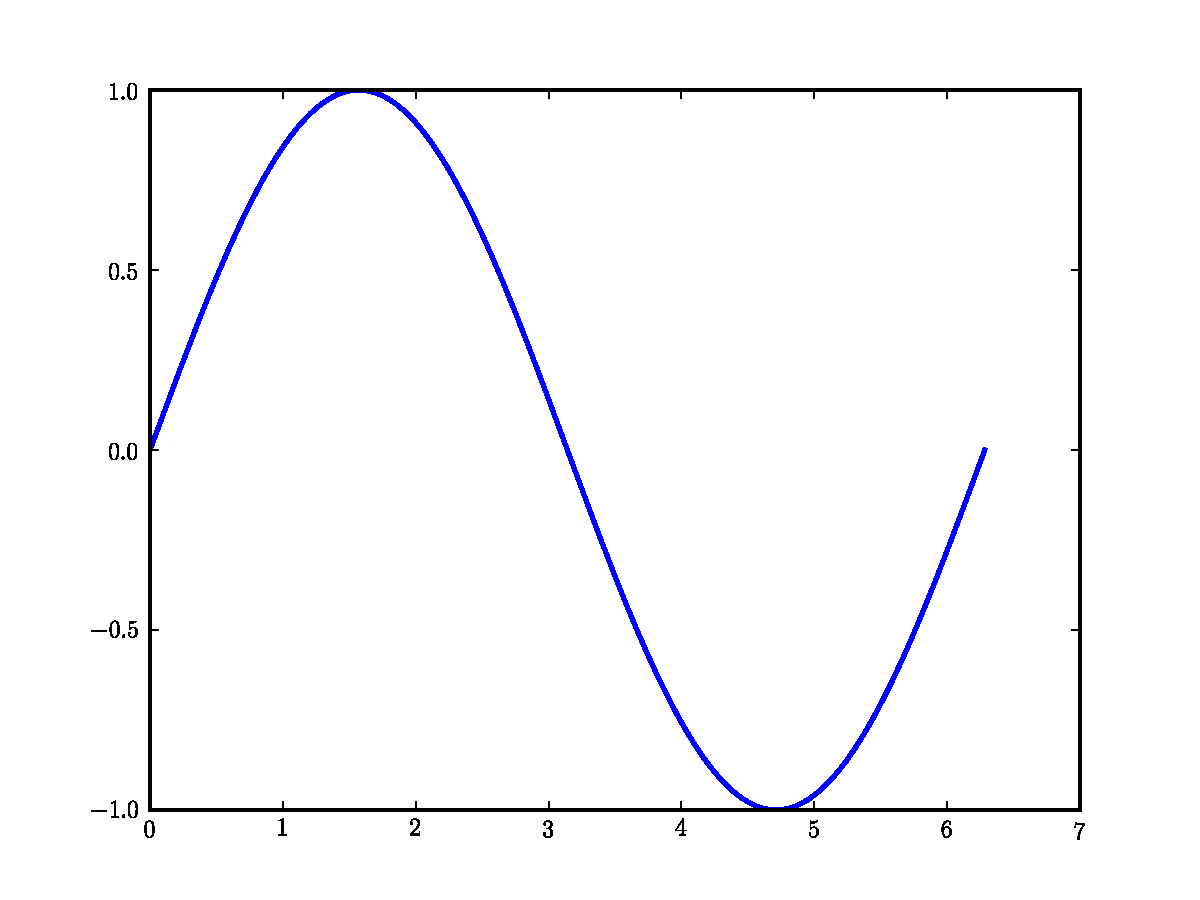
\includegraphics[width=\linewidth]{sinecurve}
    \caption{$f(x) = \sin (x)$}
\endminipage\hfill
\minipage{0.32\textwidth}
    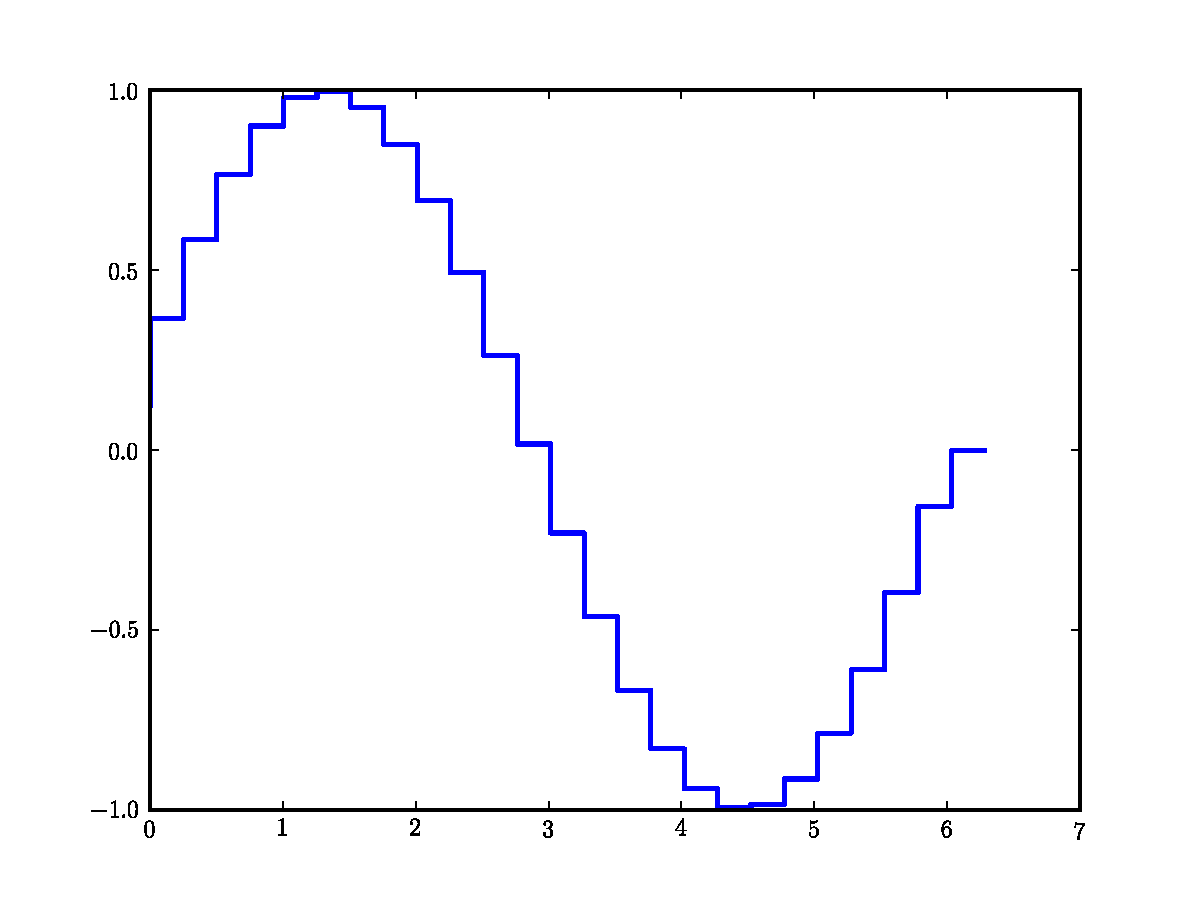
\includegraphics[width=\linewidth]{discreteSineCurve.pdf}
    \caption{$f_4$}
\endminipage\hfill
\minipage{0.32\textwidth}
    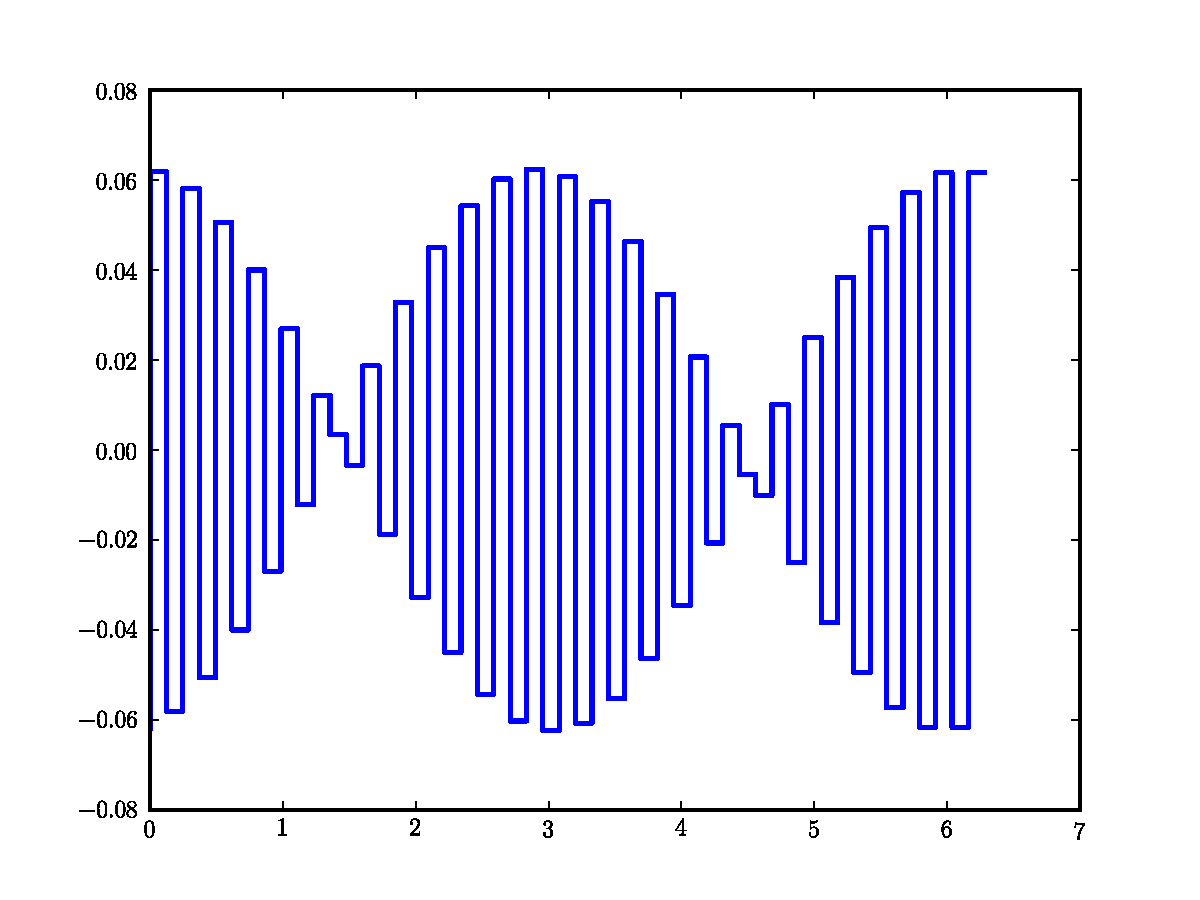
\includegraphics[width=\linewidth]{sineCurveDetail}
    \caption{$d_4$}
\endminipage
\end{figure}
\begin{problem}
Calculate and plot the approximation frames for $f(x) = \sin(x)$ on the interval $[0,2\pi]$
for $m = 4, 6, 8$. Note that because we are working on a finite interval,
we only need to calculate certain coefficients $\alpha_{m,k}$. In
particular, we only need the coefficients for $k = 0$ up to the first integer
$n$ such that $(n+1)2^{-m} > 2 \pi$ (why?). Furthermore, to plot the frame,
all we need is an array containing the relevant coefficients. Then simply plot
the coefficients against \li{linspace} with appropriate arguments
and set \li{drawstyle='steps'} in the \li{plt.plot} function.
\end{problem}

\begin{problem}
Now calculate the details for $f(x) = \sin(x)$ on the same interval and for the
same $m$ values given above. Use previous results to compute the coefficients
for $f_5$, $f_7$, and $f_9$ and plot them.
\end{problem}

What purpose do these details and approximation frames serve? According to the
properties discussed above, we can approximate $L^2$ functions as follows:
\begin{align*}
f \approx f_{J+1} &= f_J + d_J \\
&= f_{J-1} + d_{J-1} + d_J \\
& \ldots\\
&= f_{I} + d_{I} + d_{I+1} + \cdots + d_J,
\end{align*}
where $1 \leq I \leq J$. If $f$ has compact support (as in the case of a finite-time signal,
for example), only finitely many of the coefficients in the frame and the details are
nonzero, thus enabling us to represent $f$ to a reasonable degree of accuracy in a very
efficient manner. The calculation of these detail coefficients is called the \emph{discrete
wavelet transform}. In the context of signals processing, one can imagine calculating these
coefficients, transmitting them, and then reproducing the approximated signal on the
receiving end. Furthermore, the coefficients of the details reflect the local properties
of the original function $f$ at the particular level of detail and resolution! This means
that we can discard many of the coefficients if we are only interested in reproducing a certain
part of the signal, or in recovering the entire signal to only a limited resolution. We can
also study just those frequencies of the signal that fall within a certain range (called a
sub-band) by examining the detail coefficients at a particular level. These
properties make the discrete wavelet transform an attractive alternative to the Fourier
transform in many applications. See Figure \ref{fig:dwt1D} for an example of the discrete Wavelet transform.

In practice, we are often interested in analyzing discrete signals with compact support (that is,
finite-time signals that we have sampled at a finite number of points). If wavelet analysis is
to be of any use, we first need an efficient way to calculate the discrete wavelet transform.
The process described in the first section, while intuitive and illustrative of the mathematical
principles
behind wavelet analysis, is not the best approach to calculating the wavelet coefficients. It
turns out that the discrete wavelet transform can be implemented as an iterated low-pass/high-pass
filter bank, one iteration of which is shown graphically in the figure. We present the
algorithm without getting into the details of why it works.


The algorithm goes as follows.
Given an input matrix of size $2^n \times 2^n$, first operate on the rows as you would
in the one-dimensional Wavelet transform (i.e. convolve each row with the filters, then
downsample).
We then have two matrices of size $2^n \times 2^{n-1}$,
since each row has been downsampled by a factor of 2. Then for each of these two
intermediate matrices, operate on each column, yielding a total of four matrices of
size $2^{n-1} \times 2^{n-1}$. Figure \ref{fig:2dwt}
gives a graphical depiction of one iteration of the algorithm.

We initialize $LL_0$ to be the
original image matrix, and we terminate once the length of the rows or columns
is less than the length of the filters. We end up with a list of wavelet
coefficients, starting with the final approximation frame $LL_n$ followed by
collections of detail coefficients $(LH_n,HL_n,HH_n)$, $(LH_{n-1},HL_{n-1},HH_{n-1})$,
$\ldots$, $(LH_1,HL_1,HH_1)$. Note that at each iteration we operate first on the
rows (convolve with the filter, then downsample), and the we operate on the columns
of the resulting matrices (\emph{not} the original matrix). The size of the output
matrices have been reduced by a factor of two in both dimensions. As with the
one-dimensional algorithm, to reconstruct the image from the coefficients, we simply
reverse the process by upsampling, convolving, and adding (first the columns, then
the rows). We provide sample code for one iteration of the transform and the inverse.

\begin{lstlisting}
import numpy as np
from scipy.signal import fftconvolve

# given the current approximation frame image, and the filters lo_d and hi_d
# initialize empty arrays
temp = np.zeros([image.shape[0], image.shape[1]/2])
LL = np.zeros([image.shape[0]/2, image.shape[1]/2])
LH = np.zeros([image.shape[0]/2, image.shape[1]/2])
HL = np.zeros([image.shape[0]/2, image.shape[1]/2])
HH = np.zeros([image.shape[0]/2, image.shape[1]/2])

# low-pass filtering along the rows
for i in xrange(image.shape[0]):
	temp[i] = fftconvolve(image[i], lo_d, mode='full')[1::2]

# low and hi-pass filtering along the columns
for i in xrange(image.shape[1]/2):
	LL[:,i] = fftconvolve(temp[:,i],lo_d,mode='full')[1::2]
    LH[:,i] = fftconvolve(temp[:,i],hi_d,mode='full')[1::2]

# hi-pass filtering along the rows
for i in xrange(image.shape[0]):
	temp[i] = fftconvolve(image[i], hi_d, mode='full')[1::2]

# low and hi-pass filtering along the columns
for i in xrange(image.shape[1]/2):
	HL[:,i] = fftconvolve(temp[:,i],lo_d,mode='full')[1::2]
    HH[:,i] = fftconvolve(temp[:,i],hi_d,mode='full')[1::2]
\end{lstlisting}
At this point, the variables \li{LL, LH, HL, HH} contain the current level of wavelet coefficients.
You would then store \li{(LH, HL, HH)} in a list, and feed \li{LL} back into the same
block of code (with \li{LL} replacing \li{image}) to obtain the next level of coefficients.

Now, given a current level of wavelet coefficients, here is the code to recover the previous
approximation frame, which is the crucial step in the inverse transform.
\begin{lstlisting}
# given current coefficients LL, LH, HL, HH
# initialize temporary arrays
n = LL.shape[0]
temp1 = np.zeros([2*n,n])
temp2 = np.zeros([2*n,n])
up1 = np.zeros(2*n)
up2 = np.zeros(2*n)

# upsample and filter the columns of the coefficient arrays
for i in xrange(n):
	up1[1::2] = HH[:,i]
	up2[1::2] = HL[:,i]
	temp1[:,i] = fftconvolve(up1, hi_r)[1:] + fftconvolve(up2, lo_r)[1:]
	up1[1::2] = LH[:,i]
	up2[1::2] = LL[:,i]		
	temp2[:,i] = fftconvolve(up1, hi_r)[1:] + fftconvolve(up2, lo_r)[1:]

# upsample and filter the rows, then add results together
result = sp.zeros([2*n,2*n])
for i in xrange(2*n):
	up1[1::2] = temp1[i]
	up2[1::2] = temp2[i]
	result[i] = fftconvolve(up1, hi_r)[1:] + fftconvolve(up2, lo_r)[1:]
\end{lstlisting}

\begin{problem}
Build off of the sample code to fully implement the two-dimensional discrete
wavelet transform as described above.
As before, the input to your function should consist of
three arrays: the input image, the low-pass filter, and the high-pass filter.
You should return a list of the following form: $$[LL_n,(LH_n,HL_n,HH_n), \ldots
,(LH_1,HL_1,HH_1)].$$

The inverse wavelet transform function should take as input a list
of that same form, as well as the reconstruction low-pass and high-pass filters,
and should return the reconstructed image.
\end{problem}


\end{comment}